%        File: topology.tex
%     Created: Thu Nov 09 01:00 PM 2006 C
% Last Change: Thu Nov 09 01:00 PM 2006 C
%
\documentclass[a4paper]{article}
\usepackage{color,graphicx}
\usepackage{amsmath}
\usepackage{amsthm}
\usepackage{amssymb}
\usepackage{amsfonts}
\RequirePackage{ifpdf} % running on pdfTeX?
\ifpdf
\usepackage[pdftex]{hyperref}
\else
\newcommand{\href}[2]{ #1 }
\fi
\title{Netsukuku topology}
\author{http://netsukuku.freaknet.org/}
\begin{document}
\maketitle

\begin{abstract}
	This document describes the structure of the network topology of
	Netsukuku and its practical implementation.
	%%% TODO: aggiungi qualcosa in piu'
\end{abstract}

\section{Preface}
\label{sec:preface}

We're assuming that you already know the basics of the QSPN. If not, read the
QSPN document first: \cite{qspndoc}.

\section{The general idea}
\label{sec:general_idea}

The aim of Netsukuku is to be a (physical) scalable mesh network, completely
distributed and decentralised, anonymous and autonomous.

The software, which must be executed by every node of the net, has to be
unobtrusive. It has to use very few CPU and memory resources, in this way it
will be possible to run it inside low-performance computers, like Access Points,
embedded devices and old computers.

If this requirements are met, Netsukuku can be easily used to build a worldwide
distributed, anonymous and not controlled network, separated from the
Internet, without the support of any servers, ISPs or control authorities.

\section{Basic definitions}

\begin{description}
	\item[Node] We call \emph{node} any computer that is hooked up to the
		Netsukuku network.
	\item[Rnode] stands for remote node: given a node X, it is any other
		node directly linked to X, i.e. it's a neighbour of X.
	\item[Map] A map is a file, keeped by each node, whichs contains all the
		necessary information about the network, f.e. routes and nodes
		status.
\end{description}
Example:\\
\begin{figure}[h]
	\begin{center}
		\includegraphics[scale=0.5]{fig/segABC}
	\end{center}
	\caption{The nodes A,B and C}
\end{figure}
A is the rnode of B.\\
B is the rnode of A and C.\\
C is the rnode of B.

\section{Network topology}
\label{sec:net_topology}

A simple topology, which doesn't impose any structure on the network, can be
memorised with a simple map. In this map, all the information regarding the
nodes of the network have to be memorized. Surely, this kind of map cannot be
utilised by Netsukuku, because it would require too much memory.
For example, even if we store just one route to reach one node and even if
this route costs one byte, we would need 1Gb of memory for a network composed
by $10^9$ nodes (the current Internet).

For this reason, it's necessary to structure the network in a convenient
topology.

\subsection{Fractal topology}
\label{sec:fractal_topology}
\subsubsection{Level 1}
First of all we'll subdivide the network in groups of 256 nodes and we'll use
the following definitions:
\begin{description}
	\item[Gnode] means group node. It is a group of nodes, i.e. a set of
		nodes. Each node of the network belongs to just one gnode.\\
		A gnode contains a maximum of 256 nodes.
	\item[Bnode] stands for border node. It is a node which belongs to a
		gnode G, but that is also diretcly linked to at least one node
		of another gnode, i.e. some of its rnodes belongs to different
		gnodes than its.
\end{description}

Example:\\
\begin{figure}[h]
	\begin{center}
		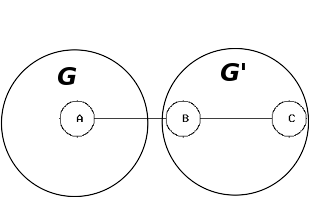
\includegraphics[scale=0.5]{fig/bnode}
	\end{center}
	\caption{The bnode A and B, belonging respectively to the gnode G and
	$G'$}
\end{figure}
A is a node belonging to the gnode G, its rnode is B.\\
B is a node belonging to the gnode $G'$, its rnode is A.\\
A is a bnode of G, while B is a bnode of $G'$.

\subsubsection{Level n}
We further subdivide the network topology in \emph{groups of 256 groups of nodes}
and we continue to name them as gnode.\\
At this point, we repeat recursively this subdivision process until
we can group all the nodes of the network into a single gnode.

Doing so, we've structured the network in $n+1$ levels (from $0$ to $n$).\\
In the base level (level 0), there are 256 single nodes.\\
In the first level (level 1), there are 256 normal gnodes. Each of them
contains 256 single nodes.\\
In the second (level 2), 256 gnodes of level 1 forms a single \emph{group of
groups of nodes}.\\
In the third (level 3), there are 256 groups of 256 groups of 256 groups of
256 nodes.\\
Continuing in this way, we arrive at the last level (level $n$), where there
is a single group which contains the whole network.\\

The QSPN algorithm is able to operate independently on any level,
considering each gnode as a single node of level 0.
For this reason, we can view the Netsukuku topology as a fractal, where each
level is composed by single nodes.

\subsubsection*{Example}

Figure \ref{fig:fract_circle}\footnote{this figure has been taken from:
\href{http://www.ian.org/FX/Plugins.html}{http://www.ian.org/FX/Plugins.html}}
is an example of the fractal topology of Netsukuku.

\begin{figure}[h]
	\begin{center}
		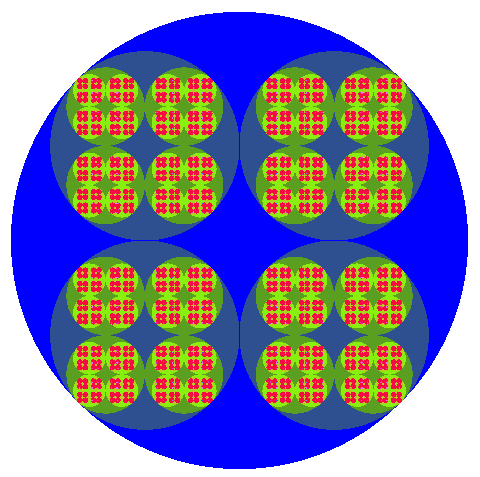
\includegraphics[scale=0.5]{fig/fractal_circle}
	\end{center}
	\caption{An example of the netsukuku topology structure}
	\label{fig:fract_circle}
\end{figure}

In this topology, each gnode contains four nodes, i.e. each group contains
four elements. The network is structured in 5 levels. The red elements, are single
nodes. The bright green circle are groups of nodes. The dark green circles are
groups of groups of nodes. The dark blue circle are groups of groups of groups of
nodes. Finally, the bright blue circle is the gnode which contains the whole
network.

\subsubsection{Membership}
Let's assign a numeric ID to each (g)gnode, starting from the last level:
\begin{enumerate}
	\item in the last level ($n$) there's only one giant gnode, thus we assign
		to it the ID ``0''. Our global ID will be:
		\[
		0
		\]
	\item in $n-1$ there are 256 gnodes, which belongs to the gnode 0 of
		level $n$, thus we assign them the IDs from $0$ to $255$.
		The global ID becomes:
		\[
		0\cdot i\quad 0\le  i\le 255
		\]
	\item we repeat the step 2 recursively gaining an ID of this form:
		\[
		0\cdot i_{n-1}\cdot i_{n-2}\cdot \dots \cdot i_0 \quad 0\le i_j\le 255,\;0\le j\le n-1
		\]
	\item since the last level is always $0$, we'll omit it and we'll
		consider only the first $n$ levels.
\end{enumerate}
In a network with a maximum of $2^32$ nodes (the maximum allowed by the ipv4),
there would be five levels ($n=4$), where each gnode will be composed by 256 nodes.
Therefore, the ID will be in the usual IP form:
\[
0\dots255\cdot 0\dots255\cdot 0\dots255\cdot 0\dots255
\]
For example, a single node of level 0 of the network is:
\[
3\cdot 41\cdot 5\cdot 12
\]
That said, each gnode of the network belongs to only one combination of gnodes
of the various levels. In our previous example we have:
\begin{align*}
	&g_3=3\\
	&g_2=41\\
	&g_1=5\\
	&g_0=12
\end{align*}
where each $g_i$ corresponds to the gnode ID of the level $i$. Note that $g_0$
is the ID attributed to the single node, at level 0.

\subsection{Fractal map}
The advantages of using a fractal topology are clear.\\
The node $N$, instead of memorising information about each node of the whole
network, will keep only that regarding the gnodes where it belongs to.
Suppose the node $N$ had this ID:
\[
g_3\cdot g_2\cdot g_1\cdot g_0
\]
It will store in memory information regarding:
\begin{enumerate}
	\item the 256 single nodes which belongs to its same gnode of level 1,
		or in other words, the 256 nodes of the gnode $g_1$,
	\item the 256 gnodes gnodes which belongs to its same gnode of level
		2, of in other words, the 256 gnodes of the gnode $g_2$,
	\item finally, the 256 gnodes which belongs to the gnode $g_3$.
\end{enumerate}
Note that doing so, the node $N$ will be blind to all the other gnodes. For
example, it won't know any information regarding the single nodes which belong
to all the other gnodes of level 1 different from $g_1$.\\

Even with this lack of knowledge, as we'll see later, the node $N$ is still
able to reach all the other nodes of the network.
In conclusion, $N$ only needs $256n$ entries in its map, instead of $2^{32}$. 
To clarify the ideas suppose that each entry costs one byte. In the plain
topology we needed $4Gb$, while in the fractal one we just need $256\cdot 4\;
b= 1Kb$.

\subsubsection{Ip v4 and v6}
Netsukuku is both compatible with ipv4 and ipv6.\\

In ipv4 there are a maximum of $2^{32}$ IPs, thus we have five levels $n=4$.\\
In ipv6 there are a maximum of $2^{128}$ IPs, thus $n=16$.

\subsubsection{Internal and external map}
For simplicity we divide the map of the node $N$, in the \emph{internal map} and in
the \emph{external} one.  The internal map contains information regarding the
nodes belonging to $g_1$. The external map describes all the other levels of
the topology.

\subsubsection{Bnode map}
The bnode map of the node $N$  contains the information regarding the bnodes
of each level where $N$ belongs.
Some examples to clarify the ideas:\\

suppose that $N = g_3\cdot g_2\cdot g_1 \cdot g_0$
\begin{itemize}
	\item a bnode of level 0 is a single node linked with two nodes of two
		different gnodes of level 1, f.e. $15, 63$.
	\item the bnodes of level 0, known by $N$, are only that which belong
		to the gnode $g_0$. Thus are all the nodes of $g_0$ which are
		linked to at least a gnode different from $g_1$.
\end{itemize}

\subsection{CIDR routing}
The QSPN, for each level, will build the routes necessary to connect each
(g)node to all the other (g)nodes of the same level. The routes will be saved
in the maps of each node.\\

If the node $N=g_3\cdot g_2\cdot g_1 \cdot g_0$ wants to reach a node $M$ which
belongs to different gnodes, f.e. $M=g_3\cdot g_2\cdot h_1 \cdot h_0$, it will
add a CIDR\cite{CIDR} route in the routing table of the kernel:\\
\emph{all the packets whose destination is $g_3\cdot g_2\cdot h_1 \cdot 0\dots
255$ will be forwarded to the gateway $X$}.\\

We'll see later how the gateway $X$ is choosen.


%bnode map
%	Size
%ext map  (sizeof)
%int map	(sizeof)
%IP addresses
%QSPN per livelli alti: chi manda chi e cosa
%			dire che all'interno del sotto gnode si diffonde come
%			un normale TP (non continuo)


%%%%%%%%%%%%%%%%
% Bibliography %
%%%%%%%%%%%%%%%%

\begin{thebibliography}{99}
	\bibitem{qspndoc} QSPN document:
		\href{http://netsukuku.freaknet.org/doc/main\_doc/qspn.pdf}{qspn.pdf}
	\bibitem{ntksite} Netsukuku website:
		\href{http://netsukuku.freaknet.org/}{http://netsukuku.freaknet.org/}
	\bibitem{CIDR} CIDR routing:
		\href{http://en.wikipedia.org/wiki/Classless\_Inter-Domain\_Routing}{Classless\_Inter-Domain\_Routing in Wikipedia}
\end{thebibliography}
\newpage

\begin{center}
\verb|^_^|
\end{center}
\end{document}
